\documentclass[]{article}

\usepackage[utf8]{inputenc}
\usepackage[usenames,dvipsnames]{xcolor}
\usepackage{fullpage}
\usepackage[upright]{fourier}
\usepackage{tkz-graph}
\usepackage{color}
\usetikzlibrary{arrows}


\usepackage[paperheight=6.2in,paperwidth=6.7in,margin=0in]{geometry}
\definecolor{color1}{RGB}{251,180,174}
\definecolor{color2}{RGB}{179,205,227}
\definecolor{color3}{RGB}{204,235,197}
\definecolor{color4}{RGB}{222,203,227}

\begin{document}
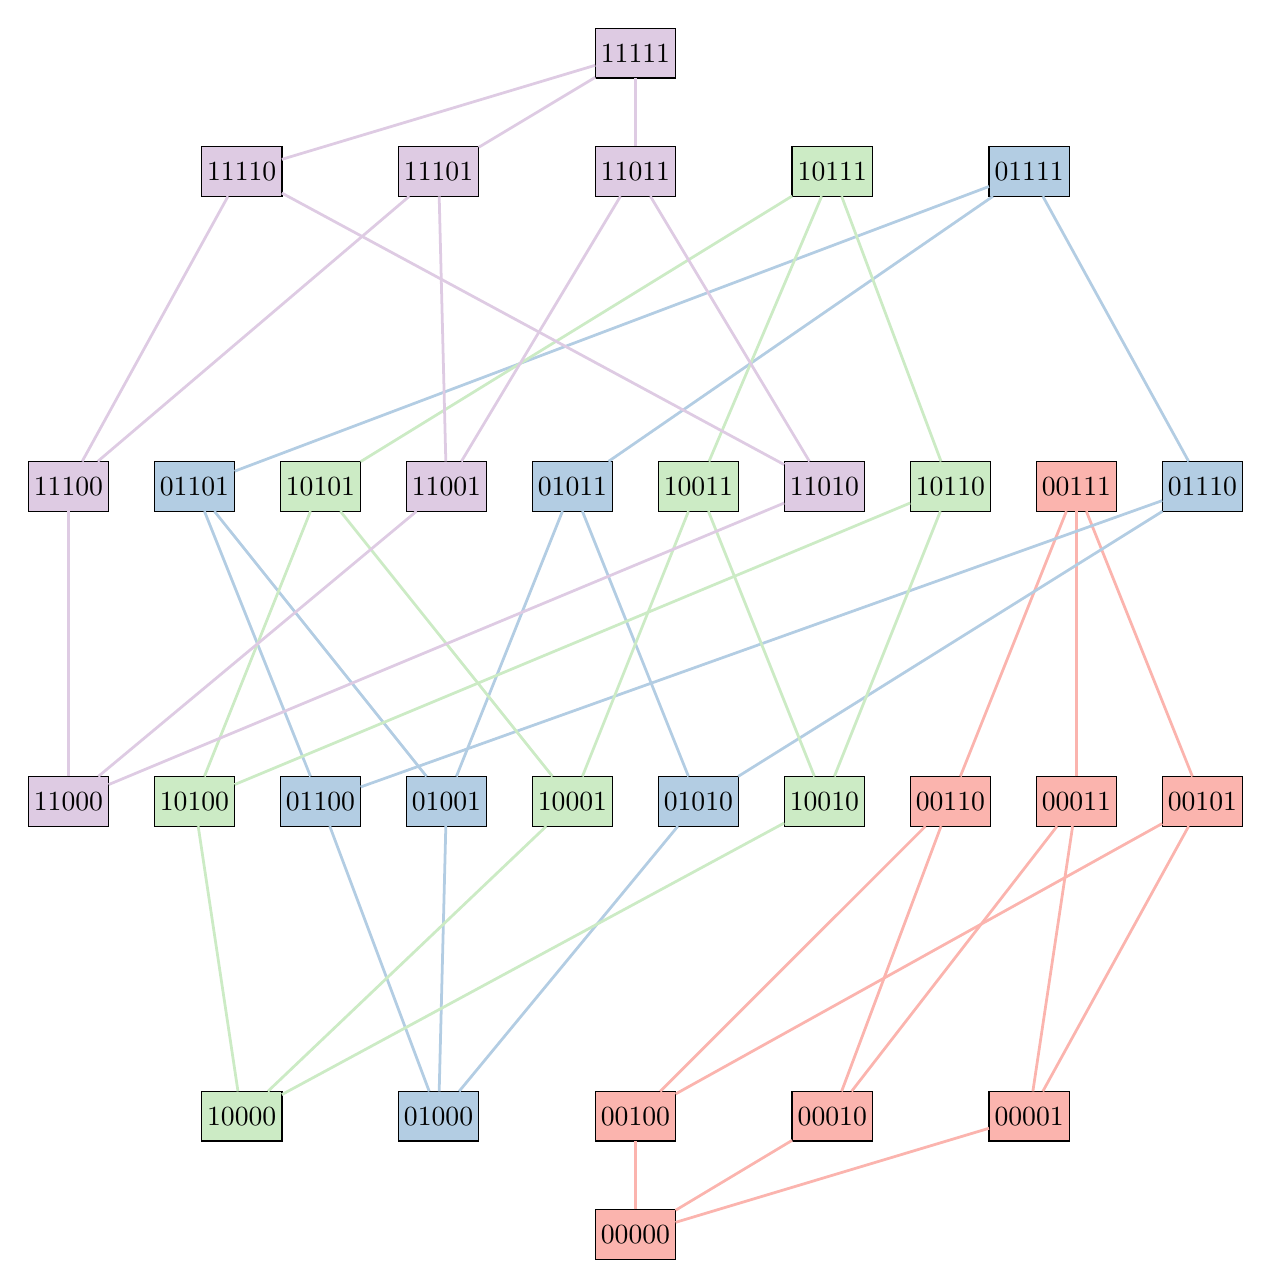
\begin{tikzpicture}
% reticulado booleano particionado com S' sendo a primeira e a segunda
% característica
  \SetVertexNormal[Shape      = rectangle,
                   FillColor  = white,
                  LineWidth  = 1pt]
  \SetUpEdge[lw         = 1pt,
             color      = black,
             labelcolor = white,
             labeltext  = red,
             labelstyle = {sloped,draw,text=blue}]

%part 00
\SetVertexNormal[Shape = rectangle, FillColor  = color1]
\Vertex[x=0, y=0, LabelOut=true, Ldist=5pt]{}
\Vertex[x=0, y=0]{$00000$}
\Vertex[x=0, y=1.5, LabelOut=true, Ldist=5pt]{}
\Vertex[x=0, y=1.5]{$00100$}
\Vertex[x=2.5, y=1.5, LabelOut=true, Ldist=5pt]{}
\Vertex[x=2.5, y=1.5]{$00010$}
\Vertex[x=5, y=1.5, LabelOut=true, Ldist=5pt]{}
\Vertex[x=5, y=1.5]{$00001$}
\Vertex[x=4.0, y=5.5, LabelOut=true, Ldist=5pt]{}
\Vertex[x=4.0, y=5.5]{$00110$}
\Vertex[x=5.6, y=5.5, LabelOut=true, Ldist=5pt]{}
\Vertex[x=5.6, y=5.5]{$00011$}
\Vertex[x=7.2, y=5.5, LabelOut=true, Ldist=5pt]{}
\Vertex[x=7.2, y=5.5]{$00101$}
\Vertex[x=5.6, y=9.5, LabelOut=true, Ldist=5pt]{}
\Vertex[x=5.6, y=9.5]{$00111$}

%part 01
\SetVertexNormal[Shape = rectangle, FillColor  = color2]
\Vertex[x=-2.5, y=1.5, LabelOut=true, Ldist=5pt]{}
\Vertex[x=-2.5, y=1.5]{$01000$}
\Vertex[x=-4.0, y=5.5, LabelOut=true, Ldist=5pt]{}
\Vertex[x=-4.0, y=5.5]{$01100$}
\Vertex[x=0.8, y=5.5, LabelOut=true, Ldist=5pt]{}
\Vertex[x=0.8, y=5.5]{$01010$}
\Vertex[x=-2.4, y=5.5, LabelOut=true, Ldist=5pt]{}
\Vertex[x=-2.4, y=5.5]{$01001$} 
\Vertex[x=-0.8, y=9.5, LabelOut=true, Ldist=5pt]{}
\Vertex[x=-0.8, y=9.5]{$01011$}
\Vertex[x=-5.6, y=9.5, LabelOut=true, Ldist=5pt]{}
\Vertex[x=-5.6, y=9.5]{$01101$}
\Vertex[x=7.2, y=9.5, LabelOut=true, Ldist=5pt]{}
\Vertex[x=7.2, y=9.5]{$01110$}
\Vertex[x=5, y=13.5, LabelOut=true, Ldist=5pt]{}
\Vertex[x=5, y=13.5]{$01111$}

%part 10
\SetVertexNormal[Shape = rectangle, FillColor  = color3]
\Vertex[x=2.4, y=5.5, LabelOut=true, Ldist=5pt]{}
\Vertex[x=2.4, y=5.5]{$10010$}
\Vertex[x=-0.8, y=5.5, LabelOut=true, Ldist=5pt]{}
\Vertex[x=-0.8, y=5.5]{$10001$}
\Vertex[x=-5, y=1.5, LabelOut=true, Ldist=5pt]{}
\Vertex[x=-5, y=1.5]{$10000$} 
\Vertex[x=-5.6, y=5.5, LabelOut=true, Ldist=5pt]{}
\Vertex[x=-5.6, y=5.5]{$10100$}
\Vertex[x=-4.0, y=9.5, LabelOut=true, Ldist=5pt]{}
\Vertex[x=-4.0, y=9.5]{$10101$}
\Vertex[x=4.0, y=9.5, LabelOut=true, Ldist=5pt]{}
\Vertex[x=4.0, y=9.5]{$10110$}
\Vertex[x=0.8, y=9.5, LabelOut=true, Ldist=5pt]{}
\Vertex[x=0.8, y=9.5]{$10011$}
\Vertex[x=2.5, y=13.5, LabelOut=true, Ldist=5pt]{}
\Vertex[x=2.5, y=13.5]{$10111$}

% part 11
\SetVertexNormal[Shape = rectangle, FillColor  = color4]
\Vertex[x=-7.2, y=5.5, LabelOut=true, Ldist=5pt]{}
\Vertex[x=-7.2, y=5.5]{$11000$}
\Vertex[x=-7.2, y=9.5, LabelOut=true, Ldist=5pt]{}
\Vertex[x=-7.2, y=9.5]{$11100$}
\Vertex[x=-2.4, y=9.5, LabelOut=true, Ldist=5pt]{}
\Vertex[x=-2.4, y=9.5]{$11001$} 
\Vertex[x=2.4, y=9.5, LabelOut=true, Ldist=5pt]{}
\Vertex[x=2.4, y=9.5]{$11010$}
\Vertex[x=-5, y=13.5, LabelOut=true, Ldist=5pt]{}
\Vertex[x=-5, y=13.5]{$11110$} 
\Vertex[x=-2.5, y=13.5, LabelOut=true, Ldist=5pt]{}
\Vertex[x=-2.5, y=13.5]{$11101$}
\Vertex[x=0, y=13.5, LabelOut=true, Ldist=5pt]{}
\Vertex[x=0, y=13.5]{$11011$}
\Vertex[x=0, y=15, LabelOut=true, Ldist=5pt]{}
\Vertex[x=0, y=15]{$11111$}

\tikzset{EdgeStyle/.style={-}}

% part 00
\SetUpEdge[lw = 1pt, color= color1]
\Edges($00000$, $00100$) 
\Edges($00000$, $00010$) 
\Edges($00000$, $00001$) 
\Edges($00100$, $00110$) 
\Edges($00100$, $00101$) 
\Edges($00010$, $00110$) 
\Edges($00010$, $00011$) 
\Edges($00101$, $00111$)
\Edges($00011$, $00111$)
\Edges($00110$, $00111$)
\Edges($00001$, $00101$) 
\Edges($00001$, $00011$) 

% part 01
\SetUpEdge[lw = 1pt, color= color2]
\Edges($01000$, $01100$) 
\Edges($01000$, $01010$) 
\Edges($01000$, $01001$) 
\Edges($01010$, $01110$)
\Edges($01010$, $01011$)
\Edges($01001$, $01101$)
\Edges($01001$, $01011$)
\Edges($01100$, $01110$)
\Edges($01100$, $01101$)
\Edges($01111$, $01011$) 
\Edges($01111$, $01101$) 
\Edges($01111$, $01110$) 

% part 10
\SetUpEdge[lw = 1pt, color= color3]
\Edges($10000$, $10100$)
\Edges($10000$, $10010$)
\Edges($10000$, $10001$)
\Edges($10100$, $10110$)
\Edges($10100$, $10101$)
\Edges($10111$, $10011$) 
\Edges($10111$, $10101$) 
\Edges($10111$, $10110$) 
\Edges($10001$, $10101$)
\Edges($10001$, $10011$)
\Edges($10010$, $10110$)
\Edges($10010$, $10011$)

% part 11
\SetUpEdge[lw = 1pt, color= color4]
\Edges($11111$, $11011$) 
\Edges($11111$, $11101$) 
\Edges($11111$, $11110$) 
\Edges($11101$, $11001$) 
\Edges($11101$, $11100$) 
\Edges($11011$, $11001$) 
\Edges($11011$, $11010$) 
\Edges($11000$, $11100$)
\Edges($11000$, $11010$)
\Edges($11000$, $11001$)
\Edges($11110$, $11010$) 
\Edges($11110$, $11100$) 

\end{tikzpicture}
\end{document}
